\documentclass[11pt]{article}

% ---------- Page setup ----------
\usepackage[margin=0.85in]{geometry}
\usepackage{fontspec}
\setmainfont{Latin Modern Roman}
\newfontfamily\bengalifont{NotoSansBengali-Regular.ttf}[Path=fonts/]
\newcommand{\bn}[1]{{\bengalifont #1}}

\usepackage{titlesec}
\usepackage{enumitem}
\usepackage{tikz}
\usetikzlibrary{arrows.meta, positioning, fit}
\usepackage[most]{tcolorbox}
\usepackage{xcolor}
\usepackage{booktabs}
\usepackage{hyperref}
\usepackage{parskip}

% ---------- Minimal, single-accent palette ----------
\definecolor{accent}{HTML}{2F5D62}   % muted teal, used sparingly
\definecolor{panel}{HTML}{F4F4F4}    % light gray fill only

\hypersetup{colorlinks=true, linkcolor=accent, urlcolor=accent, citecolor=accent}

% ---------- Compact section styling ----------
\titleformat{\section}{\large\bfseries\color{accent}}{\thesection.}{0.5em}{}
\titlespacing*{\section}{0pt}{0.9em}{0.4em}
\titleformat{\subsection}{\bfseries}{\thesubsection}{0.5em}{}
\titlespacing*{\subsection}{0pt}{0.6em}{0.2em}

\setlist{itemsep=1pt, topsep=2pt, parsep=0pt}

\pagenumbering{gobble}

\begin{document}

% ---------- Title block ----------
\begin{center}
    {\LARGE\bfseries Authorship Attribution and Style Fingerprinting\\ in Bangla Literature}\\[4pt]
    {\large\color{accent} Project Proposal}
\end{center}

\vspace{-4pt}
\hrule
\vspace{6pt}

% ---------- Overview ----------
\section{Overview and Motivation}
Authorship attribution asks: given an unseen passage, which author (from a closed candidate set) most likely wrote it, based on \emph{how} something is written rather than \emph{what} it says. Bangla literature spans stylistically distinct classical and modern voices, yet computational stylometry for Bangla remains comparatively underexplored, and per-author corpora are typically small. This project builds a multi-author Bangla stylometric pipeline that combines interpretable stylometric features with word embeddings, and directly compares a \textbf{generative} attribution paradigm against a \textbf{discriminative} one --- while also asking a representation-level question: in a small-corpus regime, do \textbf{pretrained} embeddings or embeddings \textbf{trained from scratch} on the author corpus better capture stylistic signal rather than general semantics?

% ---------- Objectives ----------
\section{Objectives}
\begin{itemize}
    \item Curate and document a cleaned, public-domain, multi-author Bangla corpus.
    \item Extract stylometric features: function-word frequencies, sentence-length distributions, POS $n$-gram statistics.
    \item Compare pretrained vs.\ from-scratch embeddings for isolating stylistic signal from semantic content.
    \item Implement and compare a generative per-author language-model attributor against a discriminative SVM / fine-tuned BERT classifier.
    \item Analyze confusion between stylistically similar authors and interpret the features driving each model's predictions.
    \item Ship a simple interface: paste a passage, receive the predicted author and the top features behind the decision.
\end{itemize}

% ---------- Methodology ----------
\section{Methodology}

\subsection{Corpus construction}
Public-domain works are collected across classical and modern Bangla authors, with sentence segmentation, normalization, deduplication, and removal of front/back matter. Sampling is balanced per author to limit corpus-size skew, and the full collection-and-cleaning process is documented as part of the methodology, not treated as a black box.

\subsection{Feature engineering}
\textbf{Stylometric:} function-word frequency vectors (pronouns, postpositions, particles), sentence-length distribution statistics (mean, variance, skew), and POS $n$-grams from a Bangla tagger.\\
\textbf{Embeddings:} (a) pretrained Bangla embeddings (e.g.\ fastText / BanglaBERT) and (b) embeddings trained from scratch on the author corpus, evaluated on how well each isolates author style versus topical content.

\subsection{Two attribution paradigms}
\textbf{Generative:} a per-author language model is fit on each author's text; an unseen passage is attributed to the author whose model assigns it the highest likelihood (lowest perplexity).\\
\textbf{Discriminative:} stylometric and embedding features are concatenated and fed to an SVM, and separately used to fine-tune a BERT classifier; both are trained directly to discriminate between authors.

\begin{center}
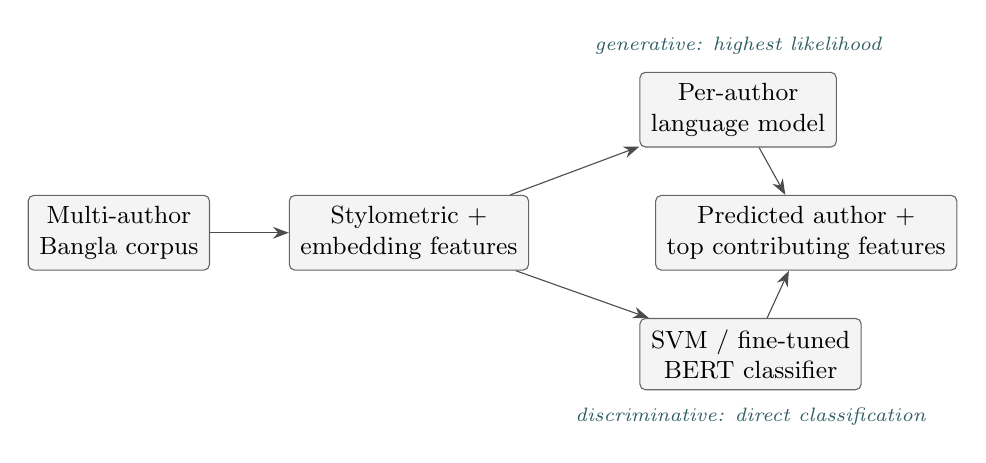
\begin{tikzpicture}[
    node distance=8mm and 10mm,
    box/.style={draw=black!60, fill=panel, rounded corners=2pt, align=center, minimum height=8mm, inner sep=4pt, font=\small},
    lbl/.style={font=\scriptsize\itshape, color=accent},
    arr/.style={-{Stealth[length=2mm]}, draw=black!70}
]
    \node[box] (corpus) {Multi-author\\Bangla corpus};
    \node[box, right=of corpus] (feat) {Stylometric +\\embedding features};

    \node[box, above right=6mm and 14mm of feat] (gen) {Per-author\\language model};
    \node[box, below right=6mm and 14mm of feat] (disc) {SVM / fine-tuned\\BERT classifier};

    \node[box, right=16mm of feat, yshift=0] (out) {Predicted author +\\top contributing features};

    \draw[arr] (corpus) -- (feat);
    \draw[arr] (feat) -- (gen);
    \draw[arr] (feat) -- (disc);
    \draw[arr] (gen) -- (out);
    \draw[arr] (disc) -- (out);

    \node[lbl, above=1mm of gen] {generative: highest likelihood};
    \node[lbl, below=1mm of disc] {discriminative: direct classification};
\end{tikzpicture}
\end{center}

\subsection{Worked example}
\begin{tcolorbox}[colback=panel, colframe=black!50, boxrule=0.4pt, arc=1mm, left=6pt, right=6pt, top=5pt, bottom=5pt]
\small
\textbf{Input passage (constructed example):} \bn{বৃষ্টি থামলে সে জানালার পাশে দাঁড়িয়ে দূরের আকাশের দিকে তাকিয়ে রইল।}\\[4pt]
\textbf{Extracted signal:} sentence length $=12$ words $\cdot$ function words \bn{পাশে}, \bn{দিকে} (postpositions), \bn{সে} (pronoun) $\cdot$ POS pattern \texttt{NOUN--VERB--ADP--NOUN}\\[4pt]
\textbf{Generative model:} log-likelihood highest under Author~B's language model.\\
\textbf{Discriminative model:} SVM assigns Author~B probability $0.71$, driven mostly by postposition frequency and mean sentence length.\\[4pt]
\textbf{Output:} \emph{Predicted author: Author~B} --- top features: postposition rate, mean sentence length, \texttt{NOUN--VERB--ADP} rate.
\end{tcolorbox}

% ---------- Evaluation ----------
\section{Evaluation Plan}
\begin{itemize}
    \item \textbf{Metrics:} accuracy and macro-F1 (per-author class imbalance), with confusion-matrix analysis focused on stylistically close authors.
    \item \textbf{Ablations:} stylometric-only vs.\ embedding-only vs.\ combined features; pretrained vs.\ from-scratch embeddings.
    \item \textbf{Interpretability:} feature-importance / SHAP for the SVM; likelihood-contribution breakdown for the generative models; comparison of which feature families drive each paradigm's correct and incorrect predictions.
\end{itemize}

% ---------- Interface ----------
\section{Interface}
A minimal input--output interface accepts a pasted Bangla passage and returns the predicted author alongside the ranked stylistic features that most influenced the decision, so predictions remain auditable rather than opaque.

% ---------- Outcomes ----------
\section{Expected Outcomes}
A documented, reusable multi-author Bangla stylometric corpus; an empirical comparison of generative and discriminative attribution for a morphologically rich, low-resource language; and evidence on whether pretrained or from-scratch embeddings better isolate authorial style in small-corpus settings.

\end{document}
